\documentclass[12pt,a4paper]{article}

\usepackage[T1]{fontenc}
\usepackage[brazilian]{babel}
\usepackage{lmodern}
\usepackage[margin=2.5cm]{geometry}
\usepackage{amsmath}
\usepackage{amssymb}
\usepackage{graphicx}
\usepackage{booktabs}
\usepackage{microtype}
\usepackage[hidelinks]{hyperref}
\usepackage{natbib}

\title{Distribuição de Ozone no conjunto de dados airquality}
\author{Guilherme Xavier}
\date{\today}

\begin{document}

\maketitle

\section{Dados}

Os dados utilizados neste relatório são provenientes do conjunto
\texttt{airquality}, disponibilizado como parte da distribuição do R.
O conjunto contém informações sobre qualidade do ar e condições
meteorológicas observadas durante os meses de maio a setembro.

A variável analisada é \textit{Ozone}, que representa a concentração de
ozônio. O conjunto possui 153 observações e 37 valores ausentes para
essa variável. A análise foi realizada com o R \citep{R2026}.

\section{Resultados}

A média mensal de \textit{Ozone} foi calculada considerando apenas os
dias em que havia uma observação disponível. A Tabela~\ref{tab:medias}
apresenta as médias mensais e o número de dias medidos em cada mês.

\begin{table}[htbp]
\centering
\caption{Média de Ozone e número de dias medidos por mês.}
\label{tab:medias}
\begin{tabular}{lrr}
\toprule
Mês & Média de Ozone & Dias medidos \\
\midrule
Maio & 23,6 & 26 \\
Junho & 29,4 & 9 \\
Julho & 59,1 & 26 \\
Agosto & 60,0 & 26 \\
Setembro & 31,4 & 29 \\
\bottomrule
\end{tabular}
\end{table}

A distribuição dos valores de \textit{Ozone} nos cinco meses é apresentada
na Figura~\ref{fig:ozone}.

\begin{figure}[htbp]
\centering
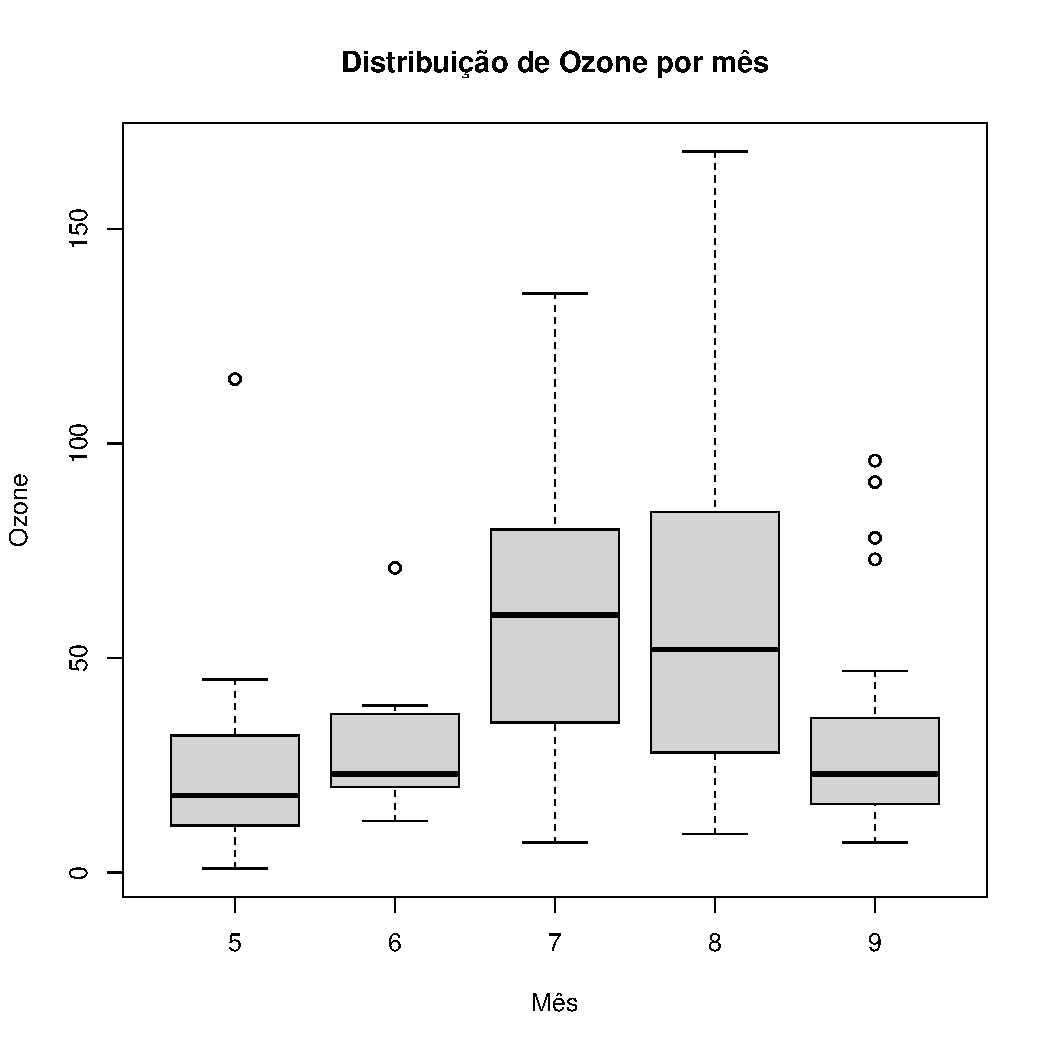
\includegraphics[width=0.85\textwidth]{figura.pdf}
\caption{Distribuição de Ozone por mês.}
\label{fig:ozone}
\end{figure}

Para cada mês, a média apresentada na Tabela~\ref{tab:medias} foi
calculada pela expressão

\begin{equation}
\bar{O}*m =
\frac{1}{n_m}
\sum*{i=1}^{n_m} O_{mi},
\label{eq:media}
\end{equation}

A expressão apresentada em~\eqref{eq:media} corresponde à média calculada pelo script.

em que $\bar{O}*m$ é a média de \textit{Ozone} no mês $m$, $O*{mi}$ é o
valor observado no dia $i$ e $n_m$ é o número de observações disponíveis
no mês. Assim, quando existem valores ausentes, o denominador conta
somente os dias que possuem um valor observado de \textit{Ozone}.

A maior média foi observada em agosto, seguida de julho, enquanto maio
apresentou a menor média entre os cinco meses. A forma de apresentação
do relatório segue a organização usual de documentos em LaTeX,
incluindo referências cruzadas para tabelas, figuras e equações
\citep{lamport1994}.

\section*{Declaração de uso de IA}

Foi utilizada a ferramenta ChatGPT como apoio durante a elaboração deste
relatório. A ferramenta foi utilizada para auxiliar na organização do
arquivo \texttt{relatorio.tex}, na construção da tabela e da equação em
LaTeX e na revisão da estrutura necessária para atender aos requisitos
do exercício. Os valores numéricos, os arquivos produzidos nos
exercícios anteriores e o resultado da compilação foram conferidos
manualmente no terminal e no próprio PDF gerado pelo \texttt{latexmk}.

\bibliographystyle{plainnat}
\bibliography{referencias}

\end{document}
